\begin{frame}{Insektvolde}

\small

\begin{columns}[T]

\begin{column}{0.58\textwidth}

\textbf{Regler for insektvolde:}

\begin{itemize}[]
\item Tilsås med tuegræsser
\item Min. 20 m mellem voldene
\item Min. 50\% soleksponeret
\item Skal kunne etableres og fjernes med landbrugsmaskiner
\item Min. 1 m bred
\end{itemize}

\vspace{0.4em}

\textbf{Gavner arter:}

\footnotesize
Vilde bier, humlebier, solitære bier, dagsommerfugle, svirrefluer, rovfugle, 
græshopper, overvintrende insekter, gul vipstjert, rødrygget tornskade, 
pirol, svaler, flagermus, pindsvin, lækat, musvåge, tårnfalk

\end{column}

\begin{column}{0.40\textwidth}
\centering
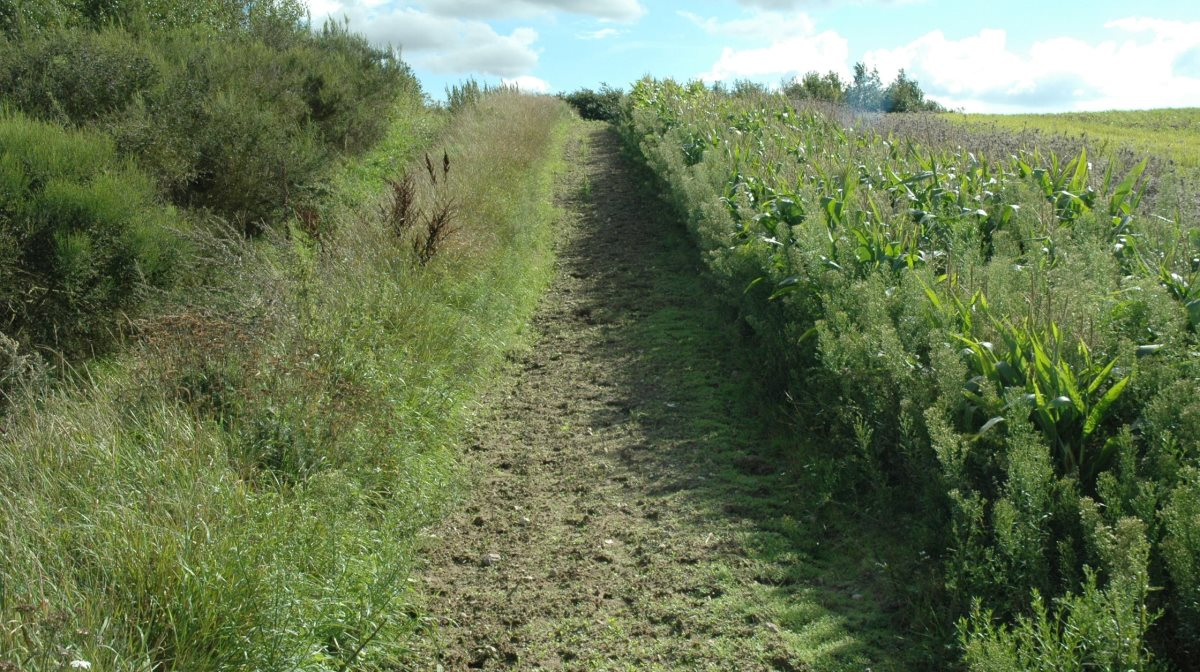
\includegraphics[width=\textwidth]{Billeder/Vildtforvaltning/biotopplantiltag/insektvold.jpg}
\end{column}

\end{columns}

\end{frame}